\section{Discussion}
% 1 page
Looking on the current state of the project, at the time of writing there is still one week left until deadline, our estimation holds more or less. We have encountered scenarios where we need do some tasks that was not defined in the beginning. Beside the extra tasks, we encountered problems with the server we made in the first part of the project, problems that could not be foreseen. The problems where mainly due to lack of proper testing of the server. When encountered with these problems, we where forced to locate if the error was in the newly created client code, or if the error originated in the server. This last part only stresses the importance of proper quality assurance.

By looking at our burndownchart (\textbf{[INSERT REF TO CHART]}) it is seen that the two lines lines up really nicely at the moment. Thou the project seems to be on track, and we should be able to reach the if we continue with this progress. Also it is seen that it is only recently that the project got back on track. This is mainly due to the extra effort needed to be made because of the problems stated in the above paragraph. Many of the problems with the server should no longer be of any concern since most of the connection with the server has been done, and therefore most of the tasks left is concerned with creating a functional GUI. \\
Beside the code, we also have to write a report for the project. A report that at this time hardly has been started - but have been split into tasks and estimated.
Even though it is primary the GUI components (beside the report) that is left to be done, extra tasks is bound to origin if we look at how is has been so far. Still, we have shown that we are able to catch up with the schedule even though we are behind. Therefore it should be possible for us to meet the deadline. In the worst case we need to downgrade some of the planned functionality or even discard some of them.

It is also appropriate to talk about how we as a group/organization developed during the project. To discuss this, we will evaluate ourselves against the Capability Maturity Model.

The Capability Maturity Model, created by the Software Engineering Institute of Carnegie Mellon University, describes the development process an organization must pass through to be considered mature.

\begin{figure}[t]
  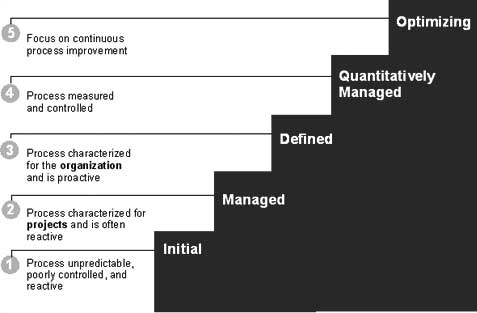
\includegraphics[width=\textwidth]{illustrations/CMM.jpg}
  \caption{Capability Maturity Model. Source: [\textit{http://www.tutorialspoint.com/cmmi/cmmi-maturity-levels.htm}]}
  \label{fig:Capability_Maturity_Model}
\end{figure}

While doing our project, we moved from the initial level of the Capability Maturity Model (while developing the server) to the managed level (during the development of the client) \cite[p. 242]{PM}. We kept to the initial level during the development of the server, by developing as we went along without using well known development methods or initial design (see figure \ref{fig:Capability_Maturity_Model}). It illuminates exactly what we want to show in this report, that using many of these tools gives us a huge advantage of producing a product, while not using any of these tools it is very uncertain any useful product can be made.

----------------------------

To be done...

- Capability Maturity Model improvement

- How well did we manage to rescue the project as seen from the current state of the project? Do it seem like we are succeeding? The report needs much work, we are barely started.
 
----------------------------

CISQ, the Consortium for IT Software Quality, is comprised by people from different parts of the software industry. It is a neutral forum for customers and suppliers of IT to define, measure and improve IT quality.

If the product fulfills the requirements and pass the tests, its \textbf{reliability} has been proved as well, which is one of CISQ's  major desirable characteristics. The other 4 are; efficiency, security, maintainability and size \cite{CISQ}

\textbf{[ TODO: Update the source if its still is needed once this has been rewritten. ]}

\begin{itemize}
	\item Efficiency means that there is minimal to none code duplication, the algorithms are optimized, etc. The code runs as smooth and fast as possible at production.
	\item Security is about how vulnerable the code is to direct attacks. If there are any obvious breaches then they affect this criteria.
	\item Maintainability: How easy is it to understand and edit the product once in production. Documented code and the clear use of known design patterns increases maintainability. 
	\item Size is not a quality indicator per see, but can be used to asses the time needed to complete the product.
\end{itemize}

How our project is measured on these five characteristics:
\begin{itemize}
 	\item The reliability of our server have been a main focus of the group. The server will continue to run after most exceptions, though the server host has been unstable and have had some irregular uptime.
 	\item The efficiency parameter comes partly from our planning and software design and partly from our implementation. This where our client differ from our server thanks to the tools we chose to use, the efficiency of the server is determined by what we found worked while coding it.
 	\item We have not prioritized security, the server does not encrypt anything. Nor is the connection between the server and client encrypted. We have deliberately chosen this as we found other elements such as streaming, more important. We acknowledge this as unacceptable if it was an actual product.  
 	\item The client is maintainable: We have a well documented and responsibility-driven product, making it easy for others to understand and maintain our code. The server is documented as well, but it is not as transparent as the client.
	\item Size can be used to determine whether we have made it too complicated. If we, from the beginning, had made interfaces for all the modules of our server, we would have seen an overly complex system, but we only discovered this after the server was almost completed. While our client seems large it is a conscious choice to lessen the complexity of the individual classes.  
\end{itemize}
\newpage